\section{Operacje na węzłach} % (fold)

W tej sekcji poznamy sposoby otrzymywania nowych obiektów z~już istniejących (rewers i~lustro splotu).
Rodzina węzłów wyposażona w~sumę spójną tworzy przemienny monoid z~jednoznacznością rozkładu.
Znacznie później (w sekcji \ref{sec:tangle}) określimy jeszcze sumę oraz iloczyn supłów.

\subsection{Lustro i~rewers} % (fold)
\begin{definition}[lustro]
    \index{lustro}
    Niech $L$ będzie zorientowanym splotem.
    Splot $mL$ powstały przez odbicie splotu $L$ względem dowolnej płaszczyzny nazywamy lustrem.
\end{definition}

\begin{definition}[rewers]
    \index{rewers}
    Niech $L$ będzie zorientowanym splotem.
    Splot $rL$ powstały przez odwrócenie orientacji wszystkich ogniw splotu $L$ nazywamy rewersem.
\end{definition}

\begin{comment}
\begin{figure}[H]
    \begin{minipage}[b]{.32\linewidth}
        \centering
        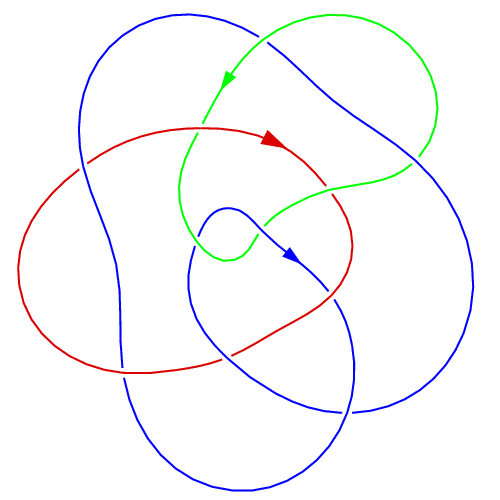
\includegraphics[width=\linewidth]{../data/link_mirror.png}
        \subcaption{lustro $mL$}
    \end{minipage}
    \begin{minipage}[b]{.32\linewidth}
        \centering
        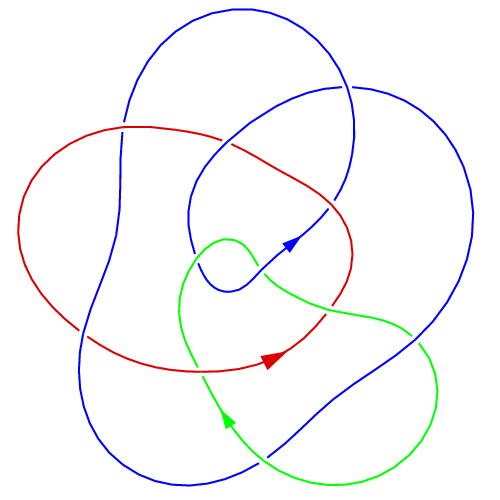
\includegraphics[width=\linewidth]{../data/link.png}
        \subcaption{przykładowy splot $L$}
    \end{minipage}
    \begin{minipage}[b]{.32\linewidth}
        \centering
        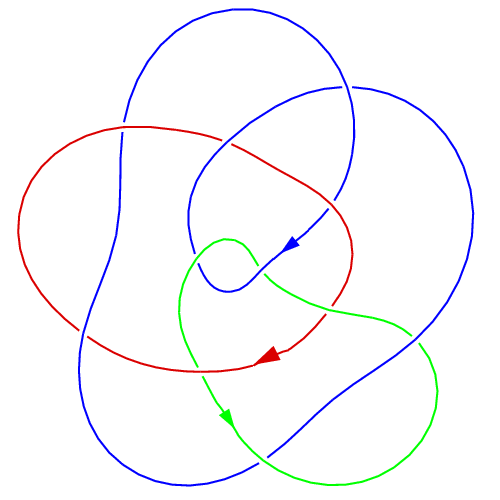
\includegraphics[width=\linewidth]{../data/link_reverse.png}
        \subcaption{rewers $rL$}
    \end{minipage}
\end{figure}
\end{comment}

Na lewym obrazku odbiliśmy diagram względem poziomej prostej, innym sposobem na otrzymanie lustra jest odwrócenie wszystkich skrzyżowań, co odpowiada odbijaniu względem płaszczyzny papieru.
Zauważmy, że wykonując powyższe operacje na węźle możemy otrzymać mniej niż czterech różne obiekty ($L$, $mL$, $rL$, $mrL$) -- na przykład trójlistnik jest własnym rewersem, ale nie lustrem.

Wyróżniamy pięć typów symetrii węzłów:

\begin{definition}[całkowicie chiralny albo skrętny]
    \index{węzeł!chiralny (skrętny)}
    Węzły $K$, $rK$, $mK$ są parami nierównoważne. % chiral 9_32
\end{definition}

\begin{definition}[odwracalny]
    \index{węzeł!odwracalny}
    Węzły $K \cong rK$ są równoważne. % reversible 3_1
\end{definition}

\begin{definition}[zwierciadlany ujemnie]
    \index{węzeł!zwierciadlany}
    Węzły $K \cong mrK$ są równoważne. % negative amphicheiral 8_17
\end{definition}

\begin{definition}[zwierciadlany dodatnio]
    Węzły $K \cong mK$ są równoważne. % positive amphicheiral 12a_427
\end{definition}

\begin{definition}[całkowicie zwierciadlany]
    Węzły $K, rK, mK$ są parami równoważne. % fully amphicheiral 4_1
\end{definition}

\begin{example}
    Węzeł $9_{32}$ jest całkowicie skrętny.
\end{example}

Całkowicie skrętne są też między innymi wszystkie węzły torusowe.

\begin{example}
    \label{exm:trefoil_is_chiral}
    Trójlistnik jest odwracalny, ale nie zwierciadlany.
\end{example}

Po raz pierwszy odkrył to M. Dehn w 1914 roku \cite{dehn14}.
Oto, jak tego dokonał.
Iloraz grafu Cayleya dla grupy podstawowej trójlistnika, $G = \pi_1(S^3 - K)$, zanurza się w~produkt $\mathbb H^2 \times \R$, co pozwala wyznaczyć grupę zewnętrznych automorfizmów grupy $G$, $\Z/2\Z$.
Korzystając z południków i równoleżników pokazał następnie, że nietrywialny automorfizm odwraca orientację przestrzeni otaczającej.
My przekonamy się o~tym przez wyznaczenie wielomianu Jonesa trójlistnika, patrz wniosek \ref{cor:joines_of_amphicheiral}.

\begin{example}
    Węzeł $8_{17}$ jest zwierciadlany ujemnie, ale nie odwracalny.
\end{example}

Sześćdziesiąt lat temu nie było pewne, czy węzły nieodwracalne w~ogóle istnieją; obecnie wiadomo, że prawie wszystkie węzły są nieodwracalne (\cite[s.~46]{murasugi96}).
W~roku 1962 Ralph Fox wskazał kilku kandydatów do tego tytułu.
Hale Trotter odkrył rok później nieskończoną rodzinę nieodwracalnych precli, patrz \ref{prp:pretzel_not_invertible}.

\begin{example}
    Węzeł $12a427$ jest zwierciadlany dodatnio, ale nie odwracalny.
\end{example}

Żaden inny węzeł pierwszy o mniej niż 13 skrzyżowaniach nie ma tej cechy.

\begin{example}
    Ósemka $4_1$ jest całkowicie zwierciadlana.
\end{example}

To najprostszy typ symetrii, wystarczy jawnie wskazać przekształcenie między diagramem węzła, jego lustra oraz odwrotności.

Tait odnosił wrażenie, że zwierciadlane węzły mają parzysty indeks skrzyżowań,
ale Hoste (Thistlethwaite?) znalazł w~1998 kontrprzykład o~piętnastu skrzyżowaniach.
Jest on jedynym znanym nam dzisiaj.
Hipoteza Taita jest prawdziwa dla węzłów pierwszych, alternujących.

Poniższa tabela oparta jest (kolejno) o~ciągi
\href{https://oeis.org/A051766}{51766},
\href{https://oeis.org/A051769}{51769},
\href{https://oeis.org/A051768}{51768},
\href{https://oeis.org/A051767}{51767},
\href{https://oeis.org/A052400}{52400},
z bazy danych ``The On-Line Encyclopedia of Integer Sequences'' (OEIS).

\begin{table}[h]
    \centering
    \begin{tabular}{@{}*{20}l@{}} \toprule
        skrzyżowania & 3 & 4 & 5 & 6 & 7 & 8 & 9 & 10 & 11 & 12 & 13 & 14 \\ \midrule
        całkowicie skrętne & 0 & 0 & 0 & 0 & 0 & 0 & 2 & 27 & 187 & 1103 & 6919 & 37885 \\
        odwracalne & 1 & 0 & 2 & 2 & 7 & 16 & 47 & 125 & 365 & 1015 & 3069 & 8813 \\
        $-$ zwierciadlane & 0 & 0 & 0 & 0 & 0 & 1 & 0 & 6 & 0 & 40 & 0 & 227 \\
        $+$ zwierciadlane & 0 & 0 & 0 & 0 & 0 & 0 & 0 & 0 & 0 & 1 & 0 & 6 \\
        zwierciadlane & 0 & 1 & 0 & 1 & 0 & 4 & 0 & 7 & 0 & 17 & 0 & 41 \\
        \bottomrule
        \hline
    \end{tabular}
    \caption{Liczba węzłów o~poszczególnych typach symetrii}

\end{table}

Można wyróżnić jeszcze jeden rodzaj symetrii.

\begin{definition}
    \label{def:period}
    \index{węzeł!okresowy}
    Węzeł $K$ nazywamy $n$-okresowym, jeśli istnieje obrót $f \colon \R^3 \to \R^3$ o~kąt $2\pi/n$ wokół pewnej prostej $l$, rozłącznej z~węzłem, taki że $f(K) = K$.
\end{definition}

Trójlistnik jest 3-okresowy, węzeł $5_1$ 5-okresowy (widać to na standardowym diagramie) i~2-okresowy.
Tę drugą symetrię można dostrzec na diagramie realizującym indeks mostowy.

\begin{proposition}
    Zbiór wszystkich okresów jest niezmiennikiem węzłów.
\end{proposition}

Z~każdym węzłem okresowym związany jest inny, prostszy węzeł.
Niech $f$ będzie obrotem z definicji \ref{def:period}, zaś $p \colon \R^3 \to \R^3/f \simeq \R^3$ rzutem na przestrzeń ilorazową.
\index{węzeł!ilorazowy}
Wtedy $p(K)$ nazywamy \emph{węzłem ilorazowym}, zaś $K$ to jego $n$-krotne nakrycie.

Murasugi podał dwa warunki, które musi spełniać węzeł o~okresie $n = p^r$, gdzie $r$ jest liczbą pierwszą.
Do ich zrozumienia potrzebujemy prostej definicji.
Ustalmy półprostą, która nie jest styczna do węzła $K$, po czym zorientujmy ją oraz węzeł.
Indeksem zaczepienia $\lambda$ węzła $p(K)$ jest różnica między liczbą skrzyżowań dodatnich oraz ujemnych wzdłuż półprostej (bez znaku).

\begin{proposition}[warunek Murasugiego]
    \index{warunek!Murasugiego}
    \label{prp:murasugi_periodic}
    Niech $K$ będzie węzłem o~okresie $n = p^r$, gdzie $p$ jest liczbą pierwszą.
    Niech $J$ będzie jego węzłem ilorazowym, z~indeksem zaczepienia $\lambda$.
    Wtedy wielomian $\alexander_J$ jest dzielnikiem wielomianu $\alexander_K$ oraz istnieje pewna całkowita liczba $k$, taka że
    \begin{equation}
        \alexander_K(t) \equiv \pm t^k \alexander_J(n)^n \left(1 + t + t^2 + \ldots + t^{\lambda - 1}\right)^{n-1} \mod p.
    \end{equation}
\end{proposition}

\begin{proof}
    Mozolne operacje na macierzach, których wyznacznikiem jest wielomian Alexandera, patrz \cite{murasugi71}.
    Kawauchi przedstawia inny dowód: najpierw dowodzi tego dla węzła torusowego $T_{n, d}$, którego węzłem ilorazowym jest niewęzeł.
    W ogólnym przypadku, korzysta z relacji kłębiastej dla wielomianu Conwaya.
    Szczegóły oraz odsyłacze do dalszych prac znaleźć można w jego przeglądowej publikacji \cite[s. 122-124]{kawauchi96}.
\end{proof}

% Koniec podsekcji Lustro i~rewers

\subsection{Suma niespójna i~suma spójna} % (fold)

Suma spójna węzłów to szczególny przypadek sklejenia dwóch rozmaitości wzdłuż brzegu.

\begin{definition}[suma niespójna]
    Niech $L_1$ oraz $L_2$ będą splotami, które leżą po różnych stronach ustalonej płaszczyzny w przestrzeni $\R^3$.
    Teoriomnogościową sumę $L_1 \sqcup L_2$ nazywamy sumą niespójną splotów.
\end{definition}

\begin{definition}[suma spójna]
    \index{suma!spójna, niespójna}
    Niech $K_1, K_2$ będą zorientowanymi węzłami.
    Natnijmy każdy z nich w dwóch punktach tego samego krótkiego łuku, a następnie zszyjmy dwoma łukami, które nie przecinają już istniejących, jak na obrazku.
    Otrzymany węzeł nazywamy sumą spójną węzłów $K_1$ oraz $K_2$.
\begin{comment}
    \[
        \begin{tikzpicture}[baseline=-0.65ex,scale=0.1]
        \begin{knot}[clip width=5, flip crossing/.list={5}, ignore endpoint intersections=false,]
            \strand[thick] (-3.5, -3.5) [in=down, out=up] to (3.5, 3.5);
            \strand[thick] (3.5, 3.5) [in=right, out=up] to (-4.5, 10);
            \strand[thick] (-4.5, 10) [in=up, out=left] to (-10, 3.5);
            \strand[thick] (-10, 3.5) to (-10, -3.5);
            \strand[thick] (-10, -3.5) [in=left, out=down] to (-4.5, -10);
            \strand[thick] (-4.5, -10) [in=down, out=right] to (3.5, -3.5);
            \strand[thick] (3.5, -3.5) [in=down, out=up] to (-3.5, 3.5);
            \strand[thick] (-3.5, 3.5) [in=left, out=up] to (4.5, 10);
            \strand[thick] (4.5, 10) [in=up, out=right] to (10, 3.5);
            \strand[thick, -Latex] (10, 3.5) to (10, -3.5);
            \strand[thick] (10, -3.5) [in=right, out=down] to (4.5, -10);
            \strand[thick] (4.5, -10) [in=down, out=left] to (-3.5, -3.5);
            \node at (0, -15) {$K_1$};
        \end{knot}
        \end{tikzpicture}
        \shrap
        \begin{tikzpicture}[baseline=-0.65ex,scale=0.1]
        \begin{knot}[clip width=5, flip crossing/.list={6}, ignore endpoint intersections=false,]
            \strand[thick] (-3.5, -3.5) [in=down, out=up] to (3.5, 3.5);
            %\strand[thick] (3.5, 3.5) [in=right, out=up] to (-4.5, 10);
            %\strand[thick] (-4.5, 10) [in=up, out=left] to (-10, 3.5);
            \strand[thick] (-10, -3.5) [in=left, out=up] to (0, 6.5);
            \strand[thick, Latex-] (-10, -3.5) [in=left, out=down] to (-4.5, -10);
            \strand[thick] (-4.5, -10) [in=down, out=right] to (3.5, -3.5);
            \strand[thick] (3.5, -3.5) [in=down, out=up] to (-3.5, 3.5);
            %\strand[thick] (-3.5, 3.5) [in=left, out=up] to (4.5, 10);
            %\strand[thick] (4.5, 10) [in=up, out=right] to (10, 3.5);
            \strand[thick] (10, -3.5) [in=right, out=up] to (0, 6.5);
            \strand[thick] (10, -3.5) [in=right, out=down] to (4.5, -10);
            \strand[thick] (4.5, -10) [in=down, out=left] to (-3.5, -3.5);
            %
            \strand[thick] (-3.5, 3.5) [in=left, out=up] to (0, 10);
            \strand[thick] (3.5, 3.5) [in=right, out=up] to (0, 10);
            \node at (0, -15) {$K_2$};
        \end{knot}
        \end{tikzpicture}
        =
        \begin{tikzpicture}[baseline=-0.65ex,scale=0.1]
        \begin{knot}[clip width=5, flip crossing/.list={5, 22, 23}, ignore endpoint intersections=false,]
            \strand[thick] (-18.5, -3.5) [in=down, out=up] to (-11.5, 3.5);
            \strand[thick] (-11.5, 3.5) [in=right, out=up] to (-19.5, 10);
            \strand[thick] (-19.5, 10) [in=up, out=left] to (-25, 3.5);
            \strand[thick] (-25, 3.5) to (-25, -3.5);
            \strand[thick] (-25, -3.5) [in=left, out=down] to (-19.5, -10);
            \strand[thick] (-19.5, -10) [in=down, out=right] to (-11.5, -3.5);
            \strand[thick] (-11.5, -3.5) [in=down, out=up] to (-18.5, 3.5);
            \strand[thick] (-18.5, 3.5) [in=left, out=up] to (-10.5, 10);
            \strand[thick] (-10.5, 10) [in=left, out=right] to (-5, 2);
            \strand[thick, -Latex] (-5, 2) to (-5+6, 2);
            \strand[thick] (5, 2) to (-5+6, 2);
            \strand[thick] (3, -2) to [in=left, out=right] (10.5, -10);
            \strand[thick, -Latex] (3, -2) to (0, -2);
            \strand[thick] (-5, -2) to (0, -2);
            \strand[thick] (-5, -2) [in=right, out=left] to (-10.5, -10);
            \strand[thick] (-10.5, -10) [in=down, out=left] to (-18.5, -3.5);
            %%%
            \strand[thick] (11.5, -3.5) [in=down, out=up] to (18.5, 3.5);
            \strand[thick] (-10 +15, 2) [in=left, out=right] to (15, 6.5);
            \strand[thick] (10.5, -10) [in=down, out=right] to (18.5, -3.5);
            \strand[thick] (18.5, -3.5) [in=down, out=up] to (11.5, 3.5);
            \strand[thick] (25, -3.5) [in=right, out=up] to (15, 6.5);
            \strand[thick] (25, -3.5) [in=right, out=down] to (19.5, -10);
            \strand[thick] (19.5, -10) [in=down, out=left] to (11.5, -3.5);
            \strand[thick] (11.5, 3.5) [in=left, out=up] to (15, 10);
            \strand[thick] (18.5, 3.5) [in=right, out=up] to (15, 10);
            %%%
            \node at (0, -15) {$K_1 \shrap K_2$};
        \end{knot}
        \end{tikzpicture}
    \]
\end{comment}
\end{definition}

\begin{tobedone}
The band sum operation is a special case of a hyperbolic transformation of a link (in 12.3) and also of a fusion of a link (in 13.1).
% Kawauchi
\end{tobedone}

Ważna jest orientacja składników: suma dwóch trójlistników może być węzłem babskim lub prostym.
Uzasadnienie, że te węzły są różne, nie jest łatwym zadaniem.
Fox pokazał w~1952 roku, że ich dopełnienia nie są homeomorficzne.
Suma przeciwnie skręconych trójlistników jest plastrowa, natomiast tak samo skręconych nie jest.
(To jedno z niewielu miejsc, gdzie nomenklatura pochodzi od żeglarzy: z~angielskiego \emph{granny knot, square knot}.)

Warunku, by zszywające łuki nie przecinały diagramów, nie można pominąć: Cromwell w~\cite[s.90]{cromwell04} pokazuje przykład dwóch niewęzłów, z~których otrzymano niepoprawnie dwie różne sumy, $6_1$ oraz $8_{20}$.

Uogólnieniem sumy spójnej oraz (nieopisanej w~naszej pracy) operacji \emph{plumbing} jest suma Murasugiego, dobrze wyjaśniona w~czwartym rozdziale książki \cite{kawauchi96}.

\begin{tobedone}
The Murasugi sum of Seifert surfaces was introduced originally in [Murasugi 1958, 1958',1958"] in order to estimate the degree of the Alexander polynomial of alter- nating links. After that, J. Stallings showed in [Stallings 1978] that a Seifert surface obtained by a Murasugi sum of fiber surfaces is a fiber surface.
\end{tobedone}

% TODO: \textbf{W topologii rozważa się podobną operację dla dwóch $n$-wymiarowych rozmaitości: z~każdej z nich usuwa się kulę, po czym skleja wzdłuż brzegu kuli. Kiedy zajmujemy się węzłami, nie interesuje nas jednak struktura rozmaitości (gdyż każdy węzeł jest równoważny z okręgiem), ale zanurzenie w~otaczającą przestrzeń.}

\begin{proposition}
    Suma spójna jest dobrze określonym działaniem.
\end{proposition}

Suma spójna nie jest dobrze określona dla splotów:
nie istnieje kanoniczny wybór, które ogniwa łączyć ze sobą.

\begin{proof}
    Niech dane będą węzły $K_1$ oraz $K_2$
    oraz dwa różne łuki $\gamma_1$, $\gamma_2$,
    których można użyć do konstrukcji sumy spójnej.
    Skurczmy $K_1$, przeciągnijmy najpierw przez łuk $\gamma_1$, a~następnie wzdłuż węzła $K_2$.
    Teraz wystarczy odwrócić ten proces z~$\gamma_2$ w~miejscu $\gamma_1$.
\end{proof}

\begin{proposition}
    Suma spójna jest działaniem łącznym oraz przemiennym.
    Niewęzeł stanowi jej element neutralny.
\end{proposition}

Prosty dowód tego faktu pozostawiamy Czytelnikowi.
W języku algebry mówimy, że węzły z~sumą spójną tworzą półgrupę (tak jak liczby naturalne z działaniem dodawania).
Dużo później pokażemy, że działaniu $\shrap$ brakuje elementów przeciwnych, więc ta struktura algebraiczna nie jest grupą.

\begin{proposition}
    Niech $K_1, K_2$ będą takimi węzłami, że $K_1 \shrap K_2 = \Unknot$. Wtedy $K_1 = K_2 = \Unknot$.
\end{proposition}

\begin{proof}[Niedowód]
    Technika ta zwana jest szwindlem Mazura.
    Załóżmy, że $K \shrap L = \Unknot$ i~dopuśćmy wyjątkowo węzły dzikie.
    Skonstruujmy sumę $K \shrap L \shrap K \shrap \ldots$,
    przy czym kolejne składniki powinny zmniejszać się,
    aby ich suma nadal była węzłem.
    Wtedy
    \begin{align*}
        K & \simeq K \shrap [(L \shrap K) \shrap (L \shrap K) \ldots] \\
         & \simeq (K \shrap L) \shrap (K \shrap L) \shrap \ldots
         \simeq \Unknot \shrap \Unknot \shrap \ldots
         \simeq \Unknot.
    \end{align*}
    Analogicznie pokazujemy, że $L \simeq \Unknot$.
\end{proof}

\begin{tobedone}
    % Kawauchi
    Theorem 3.2.1 (Non-cancellation theorem) A connected sum L1~L2 of any two links L1 and L2 is not a trivial link unless both links L1 and L2 are trivial links.
The proof (whose details are left to the reader) is essentially obtained from the following two facts:
(1) If L1 and L2 are non-split links, then L1~L2 is a non-split link.
(2) If L1~L2 is a trivial knot, then L1 and L2 are trivial knots.
(1) is directly proved by a cut-and-paste argument of combinatorial topology. (2) is usually obtained from Schubert's result on the additivity of the knot genus (cf. 4.1.5) under the connected sum, i.e., g(Ll~L2) = geLd +g(L2) (which is also proved by a cut-and-paste argument).
\end{tobedone}

Prawdziwy dowód oparty jest na topologii algebraicznej, stanowi bezpośredni wniosek z~faktów \ref{prp:genus_detects_unknot} oraz \ref{prp:genus_of_sum}.

Półgrupę węzłów z~operacją sumy spójnej można ulepszyć do grupy na dwa sposoby:
albo poprzez zmianę działania, w~jakie jest wyposażona,
albo osłabiając definicję węzłów równoważnych.
Drugi pomysł jest dużo lepszy niż pierwszy.
Na początku lat pięćdziesiątych J. Milnor wprowadził do matematyki pojęcie zgodności
(z angielskiego \emph{concordance}), które zastąpiło zwykłą równoważność.
Element neutralny nowej grupy to węzły plastrowe, ich opis leży w~sekcji \ref{sec:slice}.
Zagadnienia te zakorzenione są w~czterowymiarowej topologii.

% Koniec podsekcji Suma niespójna i~suma spójna

% Koniec sekcji Operacje na węzłach
